\chapter*{}
%\thispagestyle{empty}
%\cleardoublepage

%\thispagestyle{empty}

%\begin{titlepage}
 
 
\setlength{\centeroffset}{-0.5\oddsidemargin}
\addtolength{\centeroffset}{0.5\evensidemargin}
\thispagestyle{empty}

\noindent\hspace*{\centeroffset}\begin{minipage}{\textwidth}

\centering

 \vspace{3.3cm}

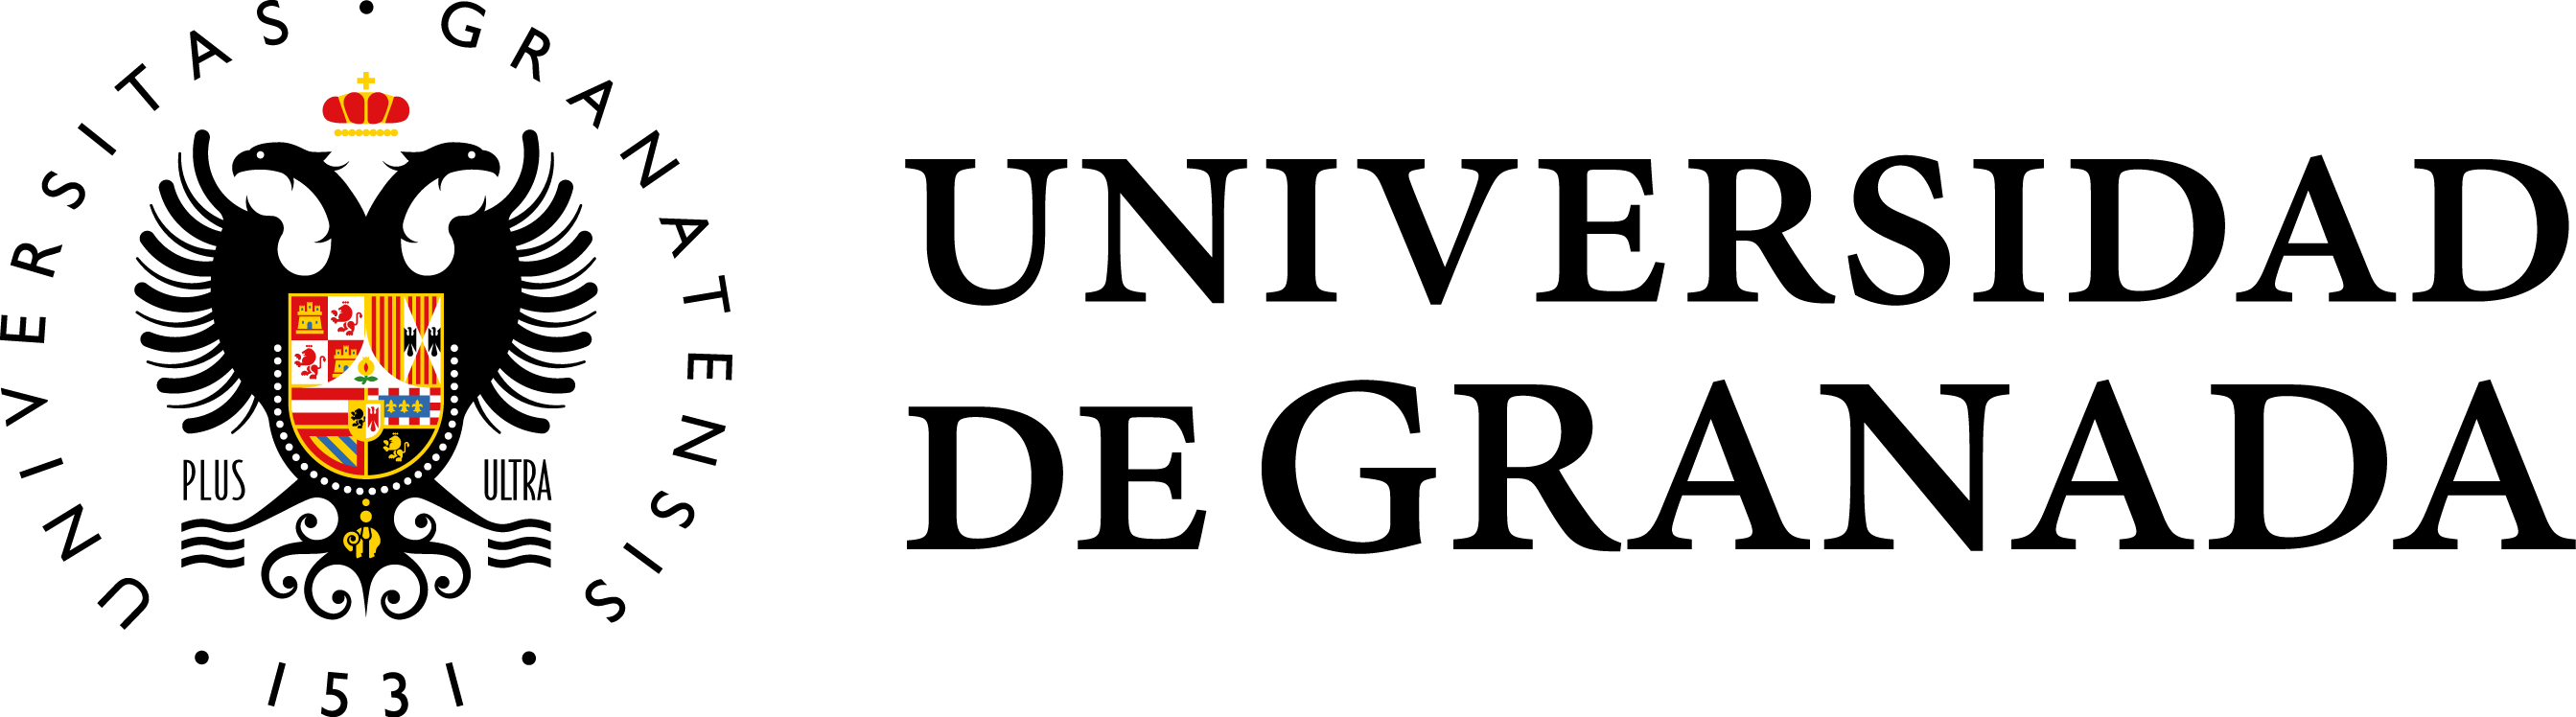
\includegraphics{imagenes/logo.png} 
 \vspace{0.5cm}

% Title

{\Huge\bfseries Criptosistemas en aplicaciones de mensajería\\
}
\noindent\rule[-1ex]{\textwidth}{3pt}\\[3.5ex]
{\large\bfseries Trabajo de fin de grado en Ingeniería Informática y Matemáticas\\[4cm]}
\end{minipage}

\vspace{2.5cm}
\noindent\hspace*{\centeroffset}\begin{minipage}{\textwidth}
\centering

\textbf{Autor}\\ {Luis Tormo Fabios}\\[2.5ex]
\textbf{Director}\\
Pedro A. García Sánchez\\
\textsc{---}\\
Granada, 7 de Septiembre de 2023
\end{minipage}

\vspace{\stretch{2}}

 
\end{titlepage}






%\cleardoublepage
%\thispagestyle{empty}

\begin{center}
{\large\bfseries Criptosistemas en aplicaciones de mensajería}\\
\end{center}
\begin{center}
Luis Tormo Fabios\\
\end{center}

%\vspace{0.7cm}
\noindent{\textbf{Palabras clave}: Criptografía simétrica, criptografía asimétrica, cuerpos finitos, intercambio de claves, curvas elípticas, funciones hash, protocolo criptográfico.}\\

\vspace{0.7cm}
\noindent{\textbf{Resumen}}\\

En esta memoria se realiza una descripción de los criptosistemas que utilizan las aplicaciones de mensajería instantáneas más populares. Para ello empiezo con un capítulo que introduce la criptografía simétrica y asimétrica. A continuación recuerdo algunos conceptos y resultados de la teoría de aritmética modular y cuerpos finitos necesaria para entender el funcionamiento de las distintas operaciones que se realizan en los distintos criptosistemas. Después describo el funcionamiento del criptosistema simétrico \emph{AES} y posteriormente describo los criptosistemas asimétricos usados, en este caso \emph{RSA} y el intercambio de claves \emph{Diffie-Hellman}. Como este tiene una versión usando Curvas Elípticas, también introduzco la teoría necesaria acerca de estas para describir su funcionamiento. Además, también dedico un capítulo a describir las funciones hash o resumen más usadas en los distintos criptosistemas. Para concluir explico el proceso criptográfico que siguen las aplicaciones de mensajería más populares e implemento una aplicación que implementa los criptosistemas más utilizados.

\cleardoublepage


\thispagestyle{empty}


\begin{center}
{\large\bfseries Cryptography in messaging app}\\
\end{center}
\begin{center}
Luis Tormo Fabios\\
\end{center}

%\vspace{0.7cm}
\noindent{\textbf{Keywords}: Symmetric cryptography, asymmetric cryptography, finite fields, key exchange, elliptic curves, hash functions, cryptographic protocol.}\\

\vspace{0.7cm}
\noindent{\textbf{Abstract}}\\

We live in an era in which social relationships cannot be conceived without thinking about social networks and in particular messaging applications. They allow us to connect, independently of physical barriers.

In this memory, the problem that I have approached has been the development of a theoretical study of the cryptosystems used by the most used messaging applications nowadays. For this purpose, I have developed in a rigorous way the mathematical and computational tools used by messaging applications. This development includes an introductory chapter in which I make an introduction to cryptography where I explain which are the objectives that cryptosystems have to fulfill to be valid and the attacks that they may be susceptible to, following the Kerchoffs principle. Then I explain the use of symmetric and asymmetric cryptosystems in instant messaging applications and I develop more extensively what symmetric cryptosystems are as well as the \emph{ECB}, \emph{CBC}, \emph{CFB} and \emph{GCM} modes of use. Finishing with an extensive development of what are the asymmetric cryptosystems.

In the next chapter, I recall some findings of modular arithmetic and finite fields necessary to understand the operation of cryptosystems such as \emph{AES} and \emph{RSA}. About modular arithmetic I develop some findings such as what is a congruence class, what are the arithmetic functions, the Chinese Remainder Theorem, findings of Euler's Phi function in particular, Euler's Theorem, and Fermat's Small Theorem among others.
On finite fields, I focus on the Galois field and the findings of this one that allows us to work with this one in a way that at a computational level to operate with this one is not so expensive than working with other fields allowing us to reduce in a significant way the computation time and the resources used.

Once the computer and mathematical tools have been introduced, I begin to explain the most widely used cryptosystems, starting with \emph{AES}.
In this chapter, I explain how \emph{AES} works. To do this I briefly introduce its history and develop its structure explaining the rounds that it performs explaining the operations that are carried out in each of them. These operations are \emph{ByteSub}, \emph{ShiftRows}, \emph{MixColumns} and \emph{AddRoundKey}. I finished the chapter explaining how the subkeys are calculated.

In the next chapter, I explain two fundamental asymmetric cryptosystems. These are \emph{RSA} and the \emph{Diffie-Hellman} key exchange protocol.
For \emph{RSA} I give a brief historical introduction and then I explain its procedures. Finally, I explain the digital signature using \emph{RSA}, a tool widely used for message validation.
For the \emph{Diffie-Hellman} key exchange I introduce \emph{The Discrete Logarithm Problem}, a problem through which the reliability of the \emph{Diffie-Hellman} key exchange is obtained. Once I saw this I explained the key exchange. Since there is a counterpart of this key exchange using \emph{Elliptic Curves} I introduce next all the theory of elliptic curves necessary to understand its operation. Once the theory is introduced I explain the \emph{Discrete Logarithm Problem} and the operation of the \emph{Diffie-Hellman} key exchange using \emph{Elliptic Curves}.

Having seen the main symmetric and asymmetric cryptosystems used by messaging applications, I have focused on explaining \emph{hash functions}.
To do this I have introduced what hash functions are and how they are constructed using the Merkle-Damgård Construction. This is a method that allows to construction of collision-resistant hash functions. Once I have seen how to build them I have described the operation of hash functions used in messaging applications. These are \emph{SHA-0}, \emph{SHA-1} and \emph{SHA-256}.

This part concludes the explanation of the computer and mathematical tools used by messaging applications and I have proceeded to explain the protocols used by the most widely used messaging applications today. 
The first protocol I developed was the \emph{MTProto protocol}, a protocol used by the Telegram messaging application. 
The next protocol I developed was \emph{the TextSecure Protocol}. Protocol used by WhatsApp, Facebook Messenger, and Signal applications among others.
Following this I have developed the protocol used by iMessage.
The last protocol I explained was \emph{Letter Sealing} used by the Line Messenger application.

Having seen this I have documented how I have developed a simple messaging application using the tools seen throughout the document. For this, I have used the \emph{Python} programming language. For this, I have used the Python programming language due to the amount of libraries it has making the work much easier. As task manager, I used \emph{PoeThePoet}, as dependency manager I used \emph{Poetry}, and as Test Runner I used \emph{Pytest}.
To create the interface I used \emph{Tkinter}, to establish the connections between devices I used the \emph{socket library}, and to create the cryptographic functions to encrypt the messages I used the \emph{Crypto library}.

Finally, I have concluded the paper with the conclusions and possible future work that I have been drawing during the development of this paper. I have also emphasized the emergence of post-quantum cryptography since in future times it will be necessary to protect our privacy since many of the current cryptosystems are vulnerable to attacks using quantum algorithms.
\chapter*{}
\thispagestyle{empty}

\noindent\rule[-1ex]{\textwidth}{2pt}\\[4.5ex]

Yo, \textbf{Luis Tormo Fabios}, alumno del doble grado de Ingeniería Informática y Matemáticas de la \textbf{Escuela Técnica Superior
de Ingenierías Informática y de Telecomunicación y la facultad de Ciencias de la Universidad de Granada}, con DNI 80169633M, autorizo la
ubicación de la siguiente copia de mi Trabajo Fin de Grado en la biblioteca del centro para que pueda ser
consultada por las personas que lo deseen.

\vspace{6cm}

\noindent Fdo: Luis Tormo Fabios

\vspace{2cm}

\begin{flushright}
Granada a X de Septiembre de 2023.
\end{flushright}


\chapter*{}
\thispagestyle{empty}

\noindent\rule[-1ex]{\textwidth}{2pt}\\[4.5ex]

D. \textbf{Pedro A. Garcı́a Sánchez}, Profesor del Área de Álgebra del Departamento Álgebra de la Universidad de Granada.

\vspace{0.5cm}

\textbf{Informan:}

\vspace{0.5cm}

Que el presente trabajo, titulado \textit{\textbf{Criptosistemas en aplicaciones de mensajería}},
ha sido realizado bajo su supervisión por \textbf{Luis Tormo Fabios}, y autorizamos la defensa de dicho trabajo ante el tribunal
que corresponda.

\vspace{0.5cm}

Y para que conste, expiden y firman el presente informe en Granada a X de Septiembre de 2023.

\vspace{1cm}

\textbf{El director:}

\vspace{5cm}

\noindent \textbf{Pedro A. Garcı́a Sánchez}

\chapter*{Agradecimientos}
\thispagestyle{empty}

       \vspace{1cm}


En primer lugar me gustaría agredecer a mi tutor del proyecto D. Pedro por su paciencia a la hora de corregir y su ayuda constante a la hora de resolver las distintas dudas y problemas que me han ido surgiendo a lo largo del desarrollo de este trabajo.\\
A todos los profesores que me han dado clase, en especial a las señoritas Isabel y Cati, Paco, Madre Andrea y D. Francisco Rojas, por confiar y enseñarme tanto.\\
A mi familia por estar presente a lo largo de estos años y en especial a mi madrina Tere y mi prima Mirian por animarme a cursar esta carrera.\\
A mi amigo Santi, porque a pesar de que dejó de estar con nosotros, nunca se fue del todo.\\
A mis abuelos, en especial a mi abuelo Juan, ya que creo que es la única persona con más ganas que yo de que termine.\\
A mis amigos, tanto a los de siempre por estar ahí todos estos años apoyándome, como  a los nuevos que me ha dado la carrera, por ser mis compañeros de fatiga. Gracias a vosotros esto ha sido mucho más fácil de llevar.\\
A Dani, Félix y Joaquín, por estar en las buenas y en las malas. Espero en los años futuros poder devolveros todo lo bueno que me habéis dado. Y si no, al menos la mitad.\\
A mis hermanos por ser uno de los motivos por los que me levanto todos los días.\\
Y por último a mis padres, por apostar por mí cuando nadie más lo hacía y no tirar la toalla, ver en mi un potencial que no sabía que tenía y aguantarme cuando no fue fácil. Si no fuera por vosotros, esto no habría sido posible.

